\documentclass[aspectratio=169,12pt,t]{beamer}

% --- Theme: Metropolis (modern, clean) ---
\usetheme[progressbar=frametitle,numbering=fraction,block=fill]{metropolis}

% --- Fira Sans font (install texlive-fonts-extra if missing) ---
\IfFileExists{FiraSans.sty}{\usepackage[sfdefault]{FiraSans}}{}

% --- Light background with warm accent ---
\definecolor{mDarkTeal}{RGB}{35,55,59}
\definecolor{mLightBrown}{RGB}{235,228,216}
\definecolor{mAccent}{RGB}{140,70,20}

\setbeamercolor{normal text}{fg=mDarkTeal,bg=white}
\setbeamercolor{alerted text}{fg=mAccent}
\setbeamercolor{frametitle}{bg=mDarkTeal,fg=white}
\setbeamercolor{progress bar}{fg=mAccent,bg=mLightBrown}
\setbeamercolor{title separator}{fg=mAccent}
\setbeamercolor{progress bar in head/foot}{fg=mAccent,bg=mLightBrown}
\setbeamercolor{progress bar in section page}{fg=mAccent,bg=mLightBrown}

% --- Packages ---
\usepackage[utf8]{inputenc}
\usepackage{amsmath,amssymb,amsthm}
\usepackage{mathrsfs}
\usepackage{tikz}
\usetikzlibrary{arrows.meta,positioning,calc,decorations.pathreplacing,shapes,patterns}
\usepackage{pgfplots}
\pgfplotsset{compat=1.18}

% --- Semi-transparent white highlight for text on top of background images ---
\usepackage[most]{tcolorbox}

% Inline highlight: \hl{short text}
\newtcbox{\hl}{%
  nobeforeafter, tcbox raise base,
  colback=white, opacityback=0.6,
  colframe=white, opacityframe=0,
  sharp corners, boxsep=2pt, left=3pt, right=3pt, top=2pt, bottom=2pt%
}

% Block highlight: \begin{hlbox} ... \end{hlbox}  (multi-line, paragraphs, itemize)
% Optional argument accepts any tcolorbox key, e.g. [width=0.6\linewidth]
\newtcolorbox{hlbox}[1][]{%
  enhanced, breakable,
  colback=white, opacityback=0.6,
  colframe=white, opacityframe=0,
  boxsep=3pt, left=6pt, right=6pt, top=4pt, bottom=4pt,
  sharp corners,
  {#1}%
}

% --- Custom colors for content types ---
\definecolor{defcolor}{RGB}{25,85,120}
\definecolor{thmcolor}{RGB}{140,35,35}
\definecolor{proofcolor}{RGB}{35,100,50}
\definecolor{excolor}{RGB}{140,75,10}
\definecolor{remcolor}{RGB}{90,90,90}

% --- Beamer blocks for mathematical content types (semi-transparent) ---
\tcbset{hlblockbase/.style={
  enhanced, breakable,
  coltitle=white, fonttitle=\bfseries,
  opacitybacktitle=0.8, opacityback=0.6,
  opacityframe=0,
  sharp corners,
  boxsep=1pt, left=5pt, right=5pt, top=2pt, bottom=2pt,
  toptitle=1pt, bottomtitle=1pt
}}

\newtcolorbox{defblock}[1]{hlblockbase, title={#1},
  colbacktitle=defcolor, colback=defcolor!15, colframe=defcolor}
\newtcolorbox{thmblock}[1]{hlblockbase, title={#1},
  colbacktitle=thmcolor, colback=thmcolor!15, colframe=thmcolor}
\newtcolorbox{proofblock}[1]{hlblockbase, title={#1},
  colbacktitle=proofcolor, colback=proofcolor!15, colframe=proofcolor}
\newtcolorbox{exblock}[1]{hlblockbase, title={#1},
  colbacktitle=excolor, colback=excolor!15, colframe=excolor}
\newtcolorbox{remblock}[1]{hlblockbase, title={#1},
  colbacktitle=remcolor, colback=remcolor!15, colframe=remcolor}

% --- Metadata ---
\title{Chapter 4: Continuity}
\subtitle{Section: Continuity and Compactness}
\author{Based on Walter Rudin's \emph{Principles of Mathematical Analysis}}
\date{}

\begin{document}

% =============================================================================
% TITLE AND OUTLINE
% =============================================================================
{
\usebackgroundtemplate{%
  
\includegraphics[width=\paperwidth,height=\paperheight,keepaspectratio=false]{chapter_04_bg_00.png}%
}
\begin{frame}[plain]
  \titlepage
  \note{
    Welcome back to Chapter 4 of Principles of Mathematical Analysis. In
    the previous sections we built up the theory of limits and continuity
    for functions between metric spaces. Now we combine continuity with
    one of the most powerful ideas from Chapter 2, namely compactness.
    The central discovery of this section is beautifully simple to state:
    a continuous function sends compact sets to compact sets. From this
    one fact we will harvest a whole crop of classical results, including
    the theorem that a continuous function on a closed bounded interval
    attains its maximum and minimum, and the theorem that continuity
    automatically upgrades to uniform continuity on a compact domain. We
    will also see, through carefully chosen counterexamples, that
    compactness really is essential to all of these results. Let's begin.
  }
\end{frame}
}

{
\usebackgroundtemplate{%
  
\includegraphics[width=\paperwidth,height=\paperheight,keepaspectratio=false]{chapter_04_bg_01.png}%
}
\begin{frame}[c]{Outline}
  \begin{center}
    \tableofcontents
  \end{center}
  \note{
    Here is our roadmap. We start with a small definition of what it means
    for a mapping into Euclidean space to be bounded. Then we prove the key
    theorem, that the continuous image of a compact set is compact. From it
    we deduce that continuous functions on compact sets are bounded and
    attain their extreme values, and that continuous one to one maps from
    compact spaces have continuous inverses. Next we introduce uniform
    continuity and show it is automatic on compact domains. Finally we show
    by example that every one of these results can fail when compactness is
    dropped.
  }
\end{frame}

% =============================================================================
\section{Motivation}
% =============================================================================

% --- Build 1/3 ---
\begin{frame}{Why Combine Continuity and Compactness?}
  \begin{hlbox}
  \begin{itemize}
    \item Continuity controls functions \alert{locally}, point by point
  \end{itemize}
  \end{hlbox}
  \note{
    So far our picture of continuity has been a local one. To check
    continuity we look at one point at a time and ask whether nearby inputs
    produce nearby outputs. This is powerful, but it is fundamentally a
    local statement. By itself it tells us very little about how a function
    behaves across its whole domain. Next, let's bring in a global idea.
  }
\end{frame}

% --- Build 2/3 ---
\begin{frame}{Why Combine Continuity and Compactness?}
  \begin{hlbox}
  \begin{itemize}
    \item Continuity controls functions \alert{locally}, point by point
    \item Compactness is a powerful \alert{global} finiteness property
  \end{itemize}
  \end{hlbox}
  \note{
    Compactness, from Chapter 2, is the global ingredient we are missing.
    Recall that a set is compact if every open cover has a finite subcover.
    This is a kind of finiteness property that lets us pass from infinitely
    many local statements to a single uniform conclusion. When we feed a
    compact set through a continuous function, something remarkable happens.
  }
\end{frame}

% --- Build 3/3 ---
\begin{frame}{Why Combine Continuity and Compactness?}
  \begin{hlbox}
  \begin{itemize}
    \item Continuity controls functions \alert{locally}, point by point
    \item Compactness is a powerful \alert{global} finiteness property
    \item Together they yield \alert{classical} theorems of analysis
  \end{itemize}

  \vspace{0.5em}
  \textbf{Preview:} extreme value theorem, continuous inverses, and
  automatic uniform continuity.
  \end{hlbox}
  \note{
    When continuity meets compactness, we get some of the most useful
    theorems in all of analysis. We will prove that a continuous real
    function on a compact set actually achieves its largest and smallest
    values. We will prove that a continuous one to one map from a compact
    space has a continuous inverse. And we will prove that continuity on a
    compact space is automatically uniform. Let's start with one small
    piece of vocabulary.
  }
\end{frame}

% =============================================================================
}

{
\usebackgroundtemplate{%
  
\includegraphics[width=\paperwidth,height=\paperheight,keepaspectratio=false]{chapter_04_bg_02.png}%
}
\section{Bounded Mappings}
% =============================================================================

\begin{frame}{Definition 4.13: Bounded Mappings}
  \begin{defblock}{Definition 4.13}
    A mapping $\mathbf{f}$ of a set $E$ into $R^k$ is \alert{bounded} if there
    is a real number $M$ such that
    \[
      |\mathbf{f}(x)| \leq M \qquad \text{for all } x \in E.
    \]
  \end{defblock}
  \vspace{0.5em}
  \begin{hlbox}
  \textbf{Idea:} the whole image $\mathbf{f}(E)$ fits inside a single ball of
  radius $M$ centered at the origin.
  \end{hlbox}
  \note{
    Here is the definition. A mapping "f" from a set "E" into "k"
    dimensional Euclidean space is called bounded if there is a single real
    number "M" so that the length of "f" of "x" never exceeds "M", no matter
    which point "x" we choose in "E". Geometrically, the entire image of the
    function sits inside one ball of radius "M" centered at the origin. This
    is a very mild looking definition, but it is exactly the property that
    our next theorems will guarantee for free when the domain is compact.
  }
\end{frame}

% =============================================================================
}

{
\usebackgroundtemplate{%
  
\includegraphics[width=\paperwidth,height=\paperheight,keepaspectratio=false]{chapter_04_bg_03.png}%
}
\section{The Key Theorem: Compactness is Preserved}
% =============================================================================

\begin{frame}{Theorem 4.14: Continuous Image of a Compact Set}
  \begin{thmblock}{Theorem 4.14}
    Suppose $f$ is a continuous mapping of a \alert{compact} metric space $X$
    into a metric space $Y$. Then $f(X)$ is \alert{compact}.
  \end{thmblock}
  \vspace{0.5em}
  \hl{\textbf{Slogan:} \emph{continuity preserves compactness.}}
  \note{
    This is the engine of the entire section. It says that if you start with
    a compact metric space "X" and push it through a continuous map "f", the
    image "f" of "X" is again compact. In a single slogan: continuity
    preserves compactness. Almost everything else in this section is a
    corollary of this one statement. Notice the proof will work directly
    with the open cover definition of compactness, rather than with
    sequences, so it is valid in any metric space. Let's look at the
    strategy first.
  }
\end{frame}

\begin{frame}{Proof Strategy: Theorem 4.14}
  \begin{hlbox}
  \textbf{Goal:} show every open cover of $f(X)$ has a finite subcover.

  \vspace{0.8em}
  \begin{enumerate}
    \item Start with an open cover $\{V_\alpha\}$ of $f(X)$.
    \item \alert{Pull back} each $V_\alpha$ to get open sets $f^{-1}(V_\alpha)$ covering $X$.
    \item Use compactness of $X$ to extract a \alert{finite} subcover.
    \item \alert{Push forward} to get finitely many $V_\alpha$ covering $f(X)$.
  \end{enumerate}
  \end{hlbox}
  \note{
    Before the details, here is the high level plan. We must show that an
    arbitrary open cover of the image has a finite subcover. The trick is to
    move the problem back to "X", where we already know compactness holds.
    We pull each open set in the cover back through "f" to get open subsets
    of "X". Continuity is exactly what makes these preimages open. They
    cover "X", so compactness of "X" gives a finite subcover. Then we push
    forward and recover finitely many original sets that cover the image.
    Pull back, use compactness, push forward. Let's carry it out.
  }
\end{frame}

% --- Build 1/3: Proof 4.14 ---
\begin{frame}{Proof of Theorem 4.14 --- Step 1: Pull Back the Cover}
  \begin{proofblock}{Step 1: Preimages are open}
    Let $\{V_\alpha\}$ be an open cover of $f(X)$. Since $f$ is continuous,
    Theorem 4.8 shows each set $f^{-1}(V_\alpha)$ is \alert{open} in $X$.
  \end{proofblock}
  \begin{center}
  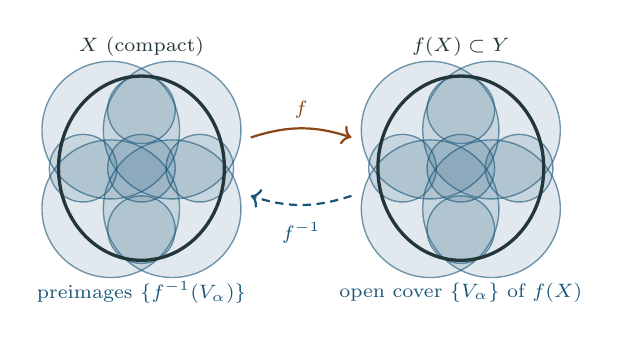
\begin{tikzpicture}[scale=0.78, every node/.style={font=\scriptsize}]
    % full open cover = many overlapping sets (4 large + 5 small) on each side
    \foreach \c in {(-0.5,0.62),(0.5,0.62),(-0.5,-0.66),(0.5,-0.66)}{
      \draw[defcolor, line width=0.5pt, fill=defcolor, fill opacity=0.13, draw opacity=0.6] \c circle (1.12);}
    \foreach \c in {(0,0.95),(0,-1.0),(-0.95,0),(0.95,0),(0,0)}{
      \draw[defcolor, line width=0.5pt, fill=defcolor, fill opacity=0.13, draw opacity=0.6] \c circle (0.55);}
    \foreach \c in {(4.7,0.62),(5.7,0.62),(4.7,-0.66),(5.7,-0.66)}{
      \draw[defcolor, line width=0.5pt, fill=defcolor, fill opacity=0.13, draw opacity=0.6] \c circle (1.12);}
    \foreach \c in {(5.2,0.95),(5.2,-1.0),(4.25,0),(6.15,0),(5.2,0)}{
      \draw[defcolor, line width=0.5pt, fill=defcolor, fill opacity=0.13, draw opacity=0.6] \c circle (0.55);}
    % the sets X and f(X) drawn on top
    \draw[very thick, mDarkTeal] (0,0) ellipse (1.35 and 1.5);
    \node[mDarkTeal] at (0,1.98) {$X$ (compact)};
    \draw[very thick, mDarkTeal] (5.2,0) ellipse (1.35 and 1.5);
    \node[mDarkTeal] at (5.2,1.98) {$f(X) \subset Y$};
    \node[defcolor] at (5.2,-2.02) {open cover $\{V_\alpha\}$ of $f(X)$};
    \node[defcolor] at (0,-2.02) {preimages $\{f^{-1}(V_\alpha)\}$};
    % arrows in the gap
    \draw[->, thick, mAccent] (1.78,0.5) to[bend left=18] (3.42,0.5);
    \node[mAccent] at (2.6,0.95) {$f$};
    \draw[->, densely dashed, thick, defcolor] (3.42,-0.45) to[bend left=18] (1.78,-0.45);
    \node[defcolor] at (2.6,-1.05) {$f^{-1}$};
  \end{tikzpicture}
  \end{center}
  \note{
    We begin the proof. Let the collection of sets "V" sub alpha be any open
    cover of the image "f" of "X". The key tool is Theorem 4.8 from the
    previous section, which characterizes continuity topologically: a map is
    continuous exactly when the preimage of every open set is open. So each
    preimage "f" inverse of "V" sub alpha is an open subset of "X". Look at
    the picture: the left oval is the compact space "X", the right oval is
    the image "f" of "X", and the many overlapping blue discs on the right
    are the cover sets. There can be a great many of them, possibly infinitely
    many. The dashed arrow labeled "f" inverse pulls each cover set back to a
    blue region inside "X", and continuity is exactly what guarantees those
    pulled back regions are open. Next we check these preimages cover all of
    "X".
  }
\end{frame}

% --- Build 2/3: Proof 4.14 ---
\begin{frame}{Proof of Theorem 4.14 --- Step 2: Finite Subcover in $X$}
  \begin{proofblock}{Step 2: Compactness of $X$}
    The sets $f^{-1}(V_\alpha)$ cover $X$. Since $X$ is compact, finitely
    many indices $\alpha_1, \dots, \alpha_n$ satisfy
    \begin{equation}
      X \subset f^{-1}(V_{\alpha_1}) \cup \cdots \cup f^{-1}(V_{\alpha_n}). \tag{12}
    \end{equation}
  \end{proofblock}
  \begin{center}
  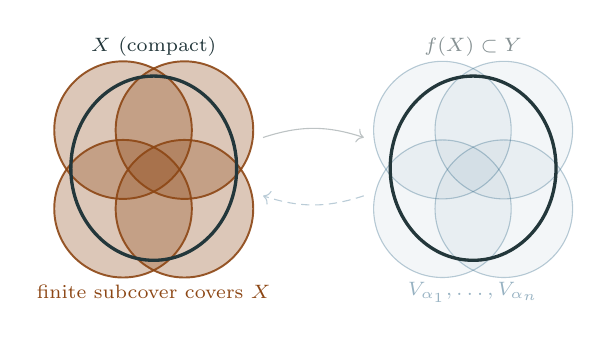
\begin{tikzpicture}[scale=0.78, every node/.style={font=\scriptsize}]
    % the chosen finite subcover -- only the 4 big sets remain
    \foreach \c in {(4.7,0.62),(5.7,0.62),(4.7,-0.66),(5.7,-0.66)}{
      \draw[defcolor, line width=0.4pt, fill=defcolor, fill opacity=0.05, draw opacity=0.3] \c circle (1.12);}
    \foreach \c in {(-0.5,0.62),(0.5,0.62),(-0.5,-0.66),(0.5,-0.66)}{
      \draw[mAccent, line width=0.7pt, fill=mAccent, fill opacity=0.3, draw opacity=0.9] \c circle (1.12);}
    \draw[very thick, mDarkTeal] (0,0) ellipse (1.35 and 1.5);
    \node[mDarkTeal] at (0,1.98) {$X$ (compact)};
    \draw[very thick, mDarkTeal] (5.2,0) ellipse (1.35 and 1.5);
    \node[mDarkTeal!55] at (5.2,1.98) {$f(X) \subset Y$};
    \node[mAccent] at (0,-2.02) {finite subcover covers $X$};
    \node[defcolor!45] at (5.2,-2.02) {$V_{\alpha_1},\dots,V_{\alpha_n}$};
    \draw[->, mDarkTeal!30] (1.78,0.5) to[bend left=18] (3.42,0.5);
    \draw[->, densely dashed, defcolor!30] (3.42,-0.45) to[bend left=18] (1.78,-0.45);
  \end{tikzpicture}
  \end{center}
  \note{
    Every point of "X" maps into the image, and the sets "V" sub alpha cover
    the image, so the preimages cover "X". Now we use the hypothesis that
    "X" is compact. By definition, the open cover of "X" by these preimages
    must contain a finite subcover. So there are finitely many indices,
    alpha one through alpha "n", whose preimages already cover "X". On the
    slide we now keep only these finitely many chosen sets, the four big
    discs highlighted in orange, and they alone already blanket all of "X".
    That is equation twelve, and it is exactly what compactness buys us.
    We have reduced an infinite cover to a finite one. Now we push this
    finiteness forward to the image.
  }
\end{frame}

% --- Build 3/3: Proof 4.14 ---
\begin{frame}{Proof of Theorem 4.14 --- Step 3: Push Forward}
  \begin{proofblock}{Step 3: Conclusion}
    Since $f(f^{-1}(E)) \subset E$ for every $E \subset Y$, relation (12) shows $f(X)$ is \alert{compact}:
    \begin{equation}
      f(X) \subset V_{\alpha_1} \cup \cdots \cup V_{\alpha_n}. \tag{13}
    \end{equation}
  \end{proofblock}
  \begin{center}
  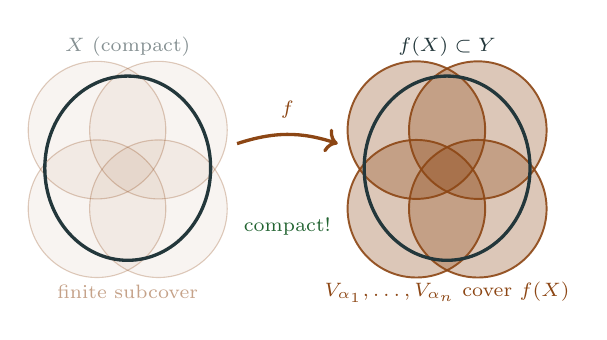
\begin{tikzpicture}[scale=0.78, every node/.style={font=\scriptsize}]
    % only the 4 big sets: faint on X, highlighted on f(X)
    \foreach \c in {(-0.5,0.62),(0.5,0.62),(-0.5,-0.66),(0.5,-0.66)}{
      \draw[mAccent, line width=0.4pt, fill=mAccent, fill opacity=0.06, draw opacity=0.28] \c circle (1.12);}
    \foreach \c in {(4.7,0.62),(5.7,0.62),(4.7,-0.66),(5.7,-0.66)}{
      \draw[mAccent, line width=0.7pt, fill=mAccent, fill opacity=0.3, draw opacity=0.9] \c circle (1.12);}
    \draw[very thick, mDarkTeal] (0,0) ellipse (1.35 and 1.5);
    \node[mDarkTeal!55] at (0,1.98) {$X$ (compact)};
    \draw[very thick, mDarkTeal] (5.2,0) ellipse (1.35 and 1.5);
    \node[mDarkTeal] at (5.2,1.98) {$f(X) \subset Y$};
    \node[mAccent!50] at (0,-2.02) {finite subcover};
    \node[mAccent] at (5.2,-2.02) {$V_{\alpha_1},\dots,V_{\alpha_n}$ cover $f(X)$};
    \draw[->, very thick, mAccent] (1.78,0.4) to[bend left=18] (3.42,0.4);
    \node[mAccent] at (2.6,0.95) {$f$};
    \node[proofcolor] at (2.6,-0.95) {compact!};
  \end{tikzpicture}
  \end{center}
  \note{
    Finally we apply "f" to both sides of equation twelve. Using the general
    set fact that "f" of the preimage of a set is contained in that set, the
    image of "X" lands inside the union of the finitely many original sets
    "V" sub alpha one through "V" sub alpha "n". On the slide the orange
    highlight has moved to the right oval: pushing the finite collection
    forward with "f", those finitely many original cover sets now blanket the
    image "f" of "X". That is equation thirteen. So we started from an
    arbitrary open cover of the image and produced a finite subcover, which
    is exactly what compactness requires. The proof is complete.
  }
\end{frame}

\begin{frame}{A Useful Set-Theoretic Remark}
  \begin{remblock}{Remark on preimages --- Equality need not hold.}
    For $E \subset Y$:\; $f(f^{-1}(E)) \subset E$.\\
    For $E \subset X$:\; $f^{-1}(f(E)) \supset E$.
  \end{remblock}
  \vspace{-1.3em}
  \begin{columns}[t]
    \column{0.5\textwidth}
    \begin{center}
    {\footnotesize $f(f^{-1}(E)) \subsetneq E$ \; ($f$ \alert{not onto})}\\[0.2em]
    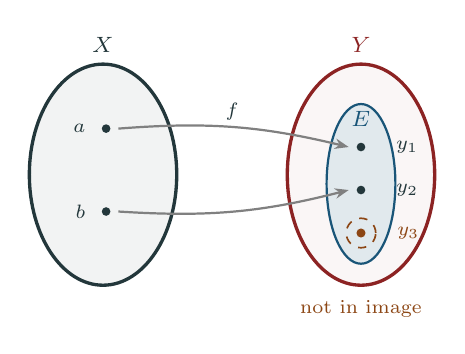
\begin{tikzpicture}[scale=0.78, >={Stealth[length=5pt]}, every node/.style={font=\scriptsize}]
      % domain X
      \draw[very thick, mDarkTeal, fill=mDarkTeal!6] (0,0) ellipse (1.2 and 1.8);
      \node[mDarkTeal, font=\footnotesize] at (0,2.12) {$X$};
      \fill[mDarkTeal] (0.05,0.75) circle (2pt);
      \node[mDarkTeal, left=4pt] at (0.05,0.75) {$a$};
      \fill[mDarkTeal] (0.05,-0.6) circle (2pt);
      \node[mDarkTeal, left=4pt] at (0.05,-0.6) {$b$};
      % target Y
      \draw[very thick, thmcolor, fill=thmcolor!4] (4.2,0) ellipse (1.2 and 1.8);
      \node[thmcolor, font=\footnotesize] at (4.2,2.12) {$Y$};
      % set E inside Y
      \draw[defcolor, thick, fill=defcolor!13] (4.2,-0.15) ellipse (0.56 and 1.3);
      \node[defcolor, font=\footnotesize] at (4.2,0.9) {$E$};
      \fill[mDarkTeal] (4.2,0.45) circle (2pt);
      \node[mDarkTeal] at (4.95,0.45) {$y_1$};
      \fill[mDarkTeal] (4.2,-0.25) circle (2pt);
      \node[mDarkTeal] at (4.95,-0.25) {$y_2$};
      \draw[mAccent, dashed, line width=0.6pt] (4.2,-0.95) circle (0.24);
      \fill[mAccent] (4.2,-0.95) circle (2.1pt);
      \node[mAccent] at (4.97,-0.95) {$y_3$};
      % arrows f (land just before the target points)
      \draw[->, gray, thick] (0.25,0.75) to[bend left=9] (4.0,0.45);
      \draw[->, gray, thick] (0.25,-0.6) to[bend right=9] (4.0,-0.25);
      \node[mDarkTeal] at (2.1,1.02) {$f$};
      \node[mAccent] at (4.2,-2.18) {not in image};
    \end{tikzpicture}
    \end{center}
    \column{0.5\textwidth}
    \begin{center}
    {\footnotesize $f^{-1}(f(E)) \supsetneq E$ \; ($f$ \alert{not 1-1})}\\[0.2em]
    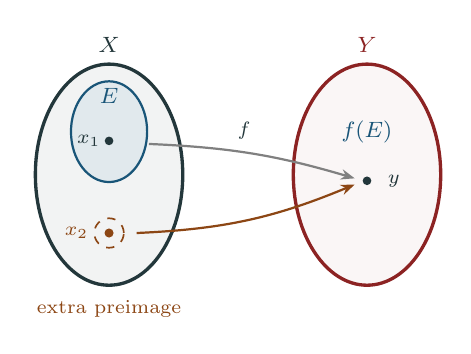
\begin{tikzpicture}[scale=0.78, >={Stealth[length=5pt]}, every node/.style={font=\scriptsize}]
      % domain X with E
      \draw[very thick, mDarkTeal, fill=mDarkTeal!6] (0,0) ellipse (1.2 and 1.8);
      \node[mDarkTeal, font=\footnotesize] at (0,2.12) {$X$};
      \draw[defcolor, thick, fill=defcolor!13] (0,0.7) ellipse (0.62 and 0.82);
      \node[defcolor, font=\footnotesize] at (0,1.28) {$E$};
      \fill[mDarkTeal] (0,0.55) circle (2pt);
      \node[mDarkTeal, left=4pt] at (0.2,0.55) {$x_1$};
      \draw[mAccent, dashed, line width=0.6pt] (0,-0.95) circle (0.24);
      \fill[mAccent] (0,-0.95) circle (2.1pt);
      \node[mAccent, left=4pt] at (0,-0.95) {$x_2$};
      % target Y with single image point
      \draw[very thick, thmcolor, fill=thmcolor!4] (4.2,0) ellipse (1.2 and 1.8);
      \node[thmcolor, font=\footnotesize] at (4.2,2.12) {$Y$};
      \fill[mDarkTeal] (4.2,-0.1) circle (2pt);
      \node[mDarkTeal, right=4pt] at (4.2,-0.1) {$y$};
      \node[defcolor, font=\footnotesize] at (4.2,0.7) {$f(E)$};
      % arrows to the same image point y (land just before it)
      \draw[->, gray, thick] (0.65,0.5) to[bend left=7] (4.0,-0.06);
      \draw[->, mAccent, thick] (0.45,-0.95) to[bend right=10] (4.0,-0.16);
      \node[mDarkTeal] at (2.2,0.72) {$f$};
      \node[mAccent] at (0,-2.18) {extra preimage};
    \end{tikzpicture}
    \end{center}
  \end{columns}
  \note{
    Let us pause on the set fact we just used, and picture why equality can
    fail. On the left, the function is not onto. The blue oval is the domain
    "X", the red oval is the target "Y", and the dashed region inside "Y" is
    our set "E", containing "y" one, "y" two, and "y" three. The arrows show
    that "X" only reaches "y" one and "y" two; nothing maps to "y" three,
    drawn in orange. So when we take the preimage of "E" and push it forward
    again, we recover only "y" one and "y" two, a strict subset of "E". That
    missed point "y" three is exactly why "f" of the preimage of "E" can be
    smaller than "E". On the right, the function is not one to one. Now "E"
    lives inside the domain and contains only "x" one. But a second point,
    "x" two, sitting outside "E" and drawn in orange, maps to the same image
    "y" as "x" one. So the image of "E" is just the single point "y", and its
    preimage pulls back both "x" one and "x" two. That extra point makes the
    preimage of the image of "E" strictly larger than "E". In short, missing
    image points shrink one side, and shared image values grow the other.
  }
\end{frame}

% =============================================================================
}

{
\usebackgroundtemplate{%
  
\includegraphics[width=\paperwidth,height=\paperheight,keepaspectratio=false]{chapter_04_bg_04.png}%
}
\section{Consequences for Real Functions}
% =============================================================================

\begin{frame}{Theorem 4.15: Closed, Bounded, and Hence Bounded}
  \begin{thmblock}{Theorem 4.15}
    If $\mathbf{f}$ is a continuous mapping of a compact metric space $X$ into
    $R^k$, then $\mathbf{f}(X)$ is \alert{closed and bounded}; thus $\mathbf{f}$
    is bounded.
  \end{thmblock}
  \vspace{0.5em}
  \begin{hlbox}
  \textbf{Why:} by Theorem 4.14, $\mathbf{f}(X)$ is compact; by Theorem 2.41,
  compact subsets of $R^k$ are closed and bounded.
  \end{hlbox}
  \note{
    Here is our first corollary. If the domain is compact and the function
    maps into "k" dimensional Euclidean space, then the image is closed and
    bounded, and in particular the function is bounded in the sense of
    Definition 4.13. The reasoning is a two step chain. First, Theorem 4.14
    tells us the image is compact. Second, the Heine Borel theorem from
    Chapter 2, Theorem 2.41, tells us that in Euclidean space compact is the
    same as closed and bounded. So the image is closed and bounded for free.
    This is especially powerful when the function is real valued.
  }
\end{frame}

\begin{frame}{Theorem 4.16: The Extreme Value Theorem}
  \begin{thmblock}{Theorem 4.16}
    Let $f$ be a continuous \alert{real} function on a compact metric space
    $X$, and set
    \[
      M = \sup_{p \in X} f(p), \qquad m = \inf_{p \in X} f(p).
    \]
    Then there exist $p, q \in X$ with $f(p) = M$ and $f(q) = m$.
  \end{thmblock}
  \vspace{0.4em}
  \begin{hlbox}
  Equivalently: $f(q) \leq f(x) \leq f(p)$ for all $x \in X$: $f$
  \alert{attains} its max and min.
  \end{hlbox}
  \note{
    This is the famous extreme value theorem, in its general metric space
    form. Let "f" be a continuous real valued function on a compact space.
    Define capital "M" to be the supremum of the values of "f", and small
    "m" to be the infimum. The theorem says these are not merely
    unattainable bounds; there are actual points "p" and "q" in the domain
    where the function equals capital "M" and small "m". In other words the
    function genuinely achieves its maximum at "p" and its minimum at "q".
    The supremum and infimum are not just approached, they are reached. Let
    me show what this looks like.
  }
\end{frame}

\begin{frame}{Visualizing the Extreme Value Theorem}
  \begin{center}
  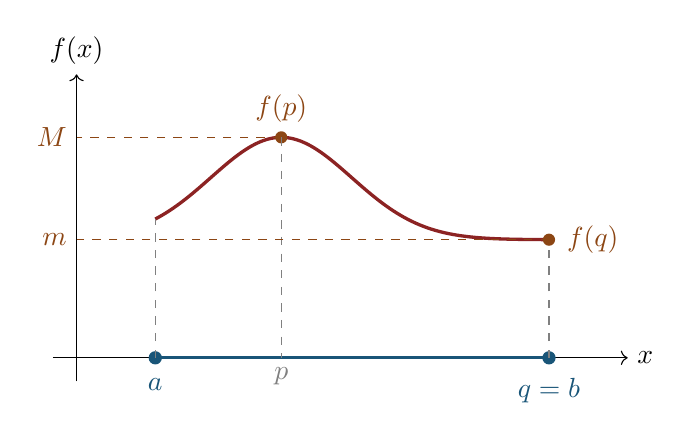
\begin{tikzpicture}[scale=1.0]
    % axes
    \draw[->] (-0.3,0) -- (7,0) node[right]{$x$};
    \draw[->] (0,-0.3) -- (0,3.6) node[above]{$f(x)$};
    % domain [a,b] drawn on the x-axis; filled endpoints = closed interval
    \draw[very thick, defcolor] (1,0) -- (6,0);
    \fill[defcolor] (1,0) circle (2.4pt);
    \fill[defcolor] (6,0) circle (2.4pt);
    \node[defcolor, below=4pt] at (1,0) {$a$};
    \node[defcolor, below=4pt] at (6,0) {$q=b$};
    % curve: interior max at x=2.6 (y=2.8), monotone down to min at x=6 (y=1.5)
    \draw[very thick, thmcolor, smooth, samples=120, domain=1:6]
      plot (\x, {1.5 + 1.3*exp(-((\x-2.6)*(\x-2.6))/1.6)});
    % dashed verticals from the endpoints up to the curve
    \draw[dashed, gray] (1,0) -- (1,1.762);
    \draw[dashed, gray] (6,0) -- (6,1.5);
    % max point (lies exactly on the curve)
    \fill[mAccent] (2.6,2.8) circle (2.2pt);
    \draw[dashed, mAccent] (2.6,2.8) -- (0,2.8) node[left]{$M$};
    \node[mAccent, above=2pt] at (2.6,2.8) {$f(p)$};
    \draw[dashed, gray] (2.6,2.8) -- (2.6,0) node[below]{$p$};
    % min point at right endpoint (lies exactly on the curve)
    \fill[mAccent] (6,1.5) circle (2.2pt);
    \draw[dashed, mAccent] (6,1.5) -- (0,1.5) node[left]{$m$};
    \node[mAccent, right=3pt] at (6,1.5) {$f(q)$};
  \end{tikzpicture}
  \end{center}
  \note{
    Look at the picture. The blue segment along the bottom is the compact
    domain, here a closed interval from "a" to "b". The two filled dots at
    "a" and "b", together with the dashed verticals running up to the curve,
    remind us that both endpoints are included, since the interval is closed.
    The dark red curve is a
    continuous function over that domain. The orange dot at the top marks
    the highest the curve ever reaches; its height is capital "M", and it
    occurs at the input "p". The other orange dot marks the lowest value,
    small "m", occurring at the input "q", which here happens to sit at the
    right endpoint. The theorem guarantees both of these dots actually exist
    on the curve. Without compactness, the curve might approach a high value
    without ever touching it; compactness is exactly what nails the dots
    down.
  }
\end{frame}

\begin{frame}{Proof of Theorem 4.16}
  \begin{proofblock}{Proof}
    By Theorem 4.15, $f(X)$ is a \alert{closed and bounded} set of real
    numbers. Hence, by Theorem 2.28, $f(X)$ contains its least upper bound
    and greatest lower bound:
    \[
      M = \sup f(X) \in f(X), \qquad m = \inf f(X) \in f(X).
    \]
    So $M$ and $m$ are values of $f$. \hfill$\blacksquare$
  \end{proofblock}
  \note{
    The proof is short because all the heavy lifting was done earlier. By
    the previous theorem, the image of "f" is a closed and bounded set of
    real numbers. Now recall Theorem 2.28 from Chapter 2: a closed and
    bounded nonempty set of real numbers contains both its supremum and its
    infimum. Apply that here. The supremum capital "M" belongs to the image,
    and the infimum small "m" belongs to the image. But belonging to the
    image means being an actual output value of "f". So there are points
    where "f" equals capital "M" and where "f" equals small "m". That is
    exactly the claim.
  }
\end{frame}

% =============================================================================
}

{
\usebackgroundtemplate{%
  
\includegraphics[width=\paperwidth,height=\paperheight,keepaspectratio=false]{chapter_04_bg_05.png}%
}
\section{Continuous Inverses}
% =============================================================================

\begin{frame}{Theorem 4.17: Continuity of the Inverse}
  \begin{thmblock}{Theorem 4.17}
    Suppose $f$ is a continuous \alert{one-to-one} mapping of a compact
    metric space $X$ \alert{onto} a metric space $Y$. Then the inverse
    mapping $f^{-1}$, defined by $f^{-1}(f(x)) = x$, is continuous on $Y$.
  \end{thmblock}
  \vspace{0.5em}
  \begin{hlbox}
  \textbf{Takeaway:} on a compact domain, a continuous bijection is
  automatically a \alert{homeomorphism}.
  \end{hlbox}
  \note{
    Our next corollary concerns inverses. Suppose "f" is continuous, one to
    one, and onto, mapping a compact space "X" onto a space "Y". A one to one
    onto map has an inverse as a function, but in general the inverse of a
    continuous map need not be continuous. This theorem says that when the
    domain is compact, that worry disappears: the inverse is automatically
    continuous. In topological language, a continuous bijection out of a
    compact space is a homeomorphism. This is an extremely handy fact. Let's
    see why it holds.
  }
\end{frame}

% --- Build 1/2: Proof 4.17 ---
\begin{frame}{Proof of Theorem 4.17 --- Step 1: From Closed to Compact}
  \begin{proofblock}{Step 1}
    By Theorem 4.8 applied to $f^{-1}$, it suffices to show $f(V)$ is open
    in $Y$ for every open $V \subset X$. Fix such a $V$.

    \medskip
    The complement $V^c$ is \alert{closed} in $X$, hence \alert{compact}
    (Theorem 2.35). Then $f(V^c)$ is a compact subset of $Y$ (Theorem 4.14).
  \end{proofblock}
  \note{
    We begin. By Theorem 4.8 applied to the inverse map, it is enough to
    show that "f" of "V" is open in "Y" whenever "V" is open in "X". So fix
    an open set "V". Its complement, written "V" complement, is closed in
    "X". Now invoke Theorem 2.35: a closed subset of a compact space is
    itself compact. So "V" complement is compact. Pushing it through "f" and
    using our main Theorem 4.14, the image of "V" complement is a compact
    subset of "Y". Next we turn compactness into closedness.
  }
\end{frame}

% --- Build 2/2: Proof 4.17 ---
\begin{frame}{Proof of Theorem 4.17 --- Step 2: Identify $f(V)$}
  \begin{proofblock}{Step 2}
    Compact subsets of $Y$ are \alert{closed} (Theorem 2.34), so $f(V^c)$ is
    closed. Since $f$ is one-to-one and onto,
    \[
      f(V) = \big(f(V^c)\big)^c .
    \]
    The complement of a closed set is open, so $f(V)$ is \alert{open}. \hfill$\blacksquare$
  \end{proofblock}
  \note{
    By Theorem 2.34, every compact subset of a metric space is closed, so
    the image of "V" complement is a closed set in "Y". Now we use that "f"
    is a bijection. Because "f" is one to one and onto, it sends complements
    to complements: the image of "V" is exactly the complement of the image
    of "V" complement. We just showed that latter set is closed, and the
    complement of a closed set is open. Therefore the image of "V" is open.
    Since "V" was an arbitrary open set, this proves the inverse is
    continuous, completing the proof.
  }
\end{frame}

% =============================================================================
}

{
\usebackgroundtemplate{%
  
\includegraphics[width=\paperwidth,height=\paperheight,keepaspectratio=false]{chapter_04_bg_06.png}%
}
\section{Uniform Continuity}
% =============================================================================

\begin{frame}{Definition 4.18: Uniform Continuity}
  \begin{defblock}{Definition 4.18}
    $f : X \to Y$ is \alert{uniformly continuous} on $X$ if for every
    $\varepsilon > 0$ there exists $\delta > 0$ such that
    \[
      d_Y(f(p), f(q)) < \varepsilon \quad\text{whenever}\quad d_X(p,q) < \delta,
    \]
    for \alert{all} $p, q \in X$.
  \end{defblock}
  \vspace{0.4em}
  \begin{hlbox}
  The same $\delta$ works \emph{everywhere} --- it depends on $\varepsilon$
  only, not on the point.
  \end{hlbox}
  \note{
    Now a new and stronger concept. A function is uniformly continuous on
    "X" if for every epsilon greater than zero there is a delta greater than
    zero so that whenever two points "p" and "q" are within delta of each
    other, their images are within epsilon. The phrase to focus on is for
    all "p" and "q". A single delta must work simultaneously for every pair
    of nearby points across the entire space. Compare this with ordinary
    continuity, where delta is allowed to depend on the particular point you
    are sitting at. Here delta depends on epsilon alone. To build intuition,
    let us first picture what this uniform behavior looks like.
  }
\end{frame}

\begin{frame}{Visualizing Uniform Continuity}
  \begin{center}
  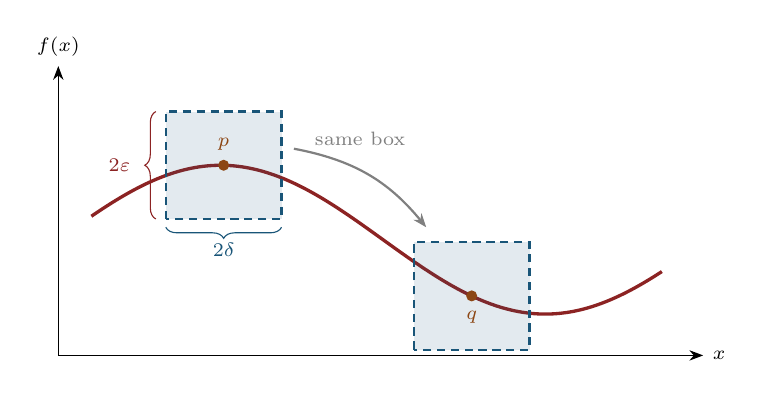
\begin{tikzpicture}[scale=1.05, >={Stealth[length=5pt]}, every node/.style={font=\scriptsize}]
    % axes
    \draw[->] (0,0) -- (7.8,0) node[right]{$x$};
    \draw[->] (0,0) -- (0,3.5) node[above]{$f(x)$};
    % curve (bounded slope -> uniformly continuous)
    \draw[very thick, thmcolor, smooth, samples=160, domain=0.4:7.3]
      plot (\x, {1.4 + 0.9*sin(deg(0.8*\x))});
    % --- Box 1 at p (width 2*delta, height 2*eps) ---
    \fill[defcolor, fill opacity=0.12] (1.3,1.65) rectangle (2.7,2.95);
    \draw[defcolor, thick, densely dashed] (1.3,1.65) rectangle (2.7,2.95);
    \fill[mAccent] (2.0,2.30) circle (1.9pt);
    \node[mAccent, above=2pt] at (2.0,2.30) {$p$};
    \draw[decorate, decoration={brace, amplitude=4pt, mirror}, defcolor]
      (1.3,1.55) -- (2.7,1.55);
    \node[defcolor] at (2.0,1.28) {$2\delta$};
    \draw[decorate, decoration={brace, amplitude=4pt}, thmcolor]
      (1.18,1.65) -- (1.18,2.95);
    \node[thmcolor] at (0.74,2.3) {$2\varepsilon$};
    % --- Box 2 at q: SAME size, different location ---
    \fill[defcolor, fill opacity=0.12] (4.3,0.07) rectangle (5.7,1.37);
    \draw[defcolor, thick, densely dashed] (4.3,0.07) rectangle (5.7,1.37);
    \fill[mAccent] (5.0,0.72) circle (1.9pt);
    \node[mAccent, below=2pt] at (5.0,0.72) {$q$};
    % connect: same box slides
    \draw[->, gray, thick] (2.85,2.5) to[bend left=20] (4.45,1.55);
    \node[gray] at (3.65,2.62) {same box};
  \end{tikzpicture}
  \end{center}
  \vspace{0.1em}
  \begin{hlbox}
  {\footnotesize Fix $\varepsilon$. One $\delta$ gives a box of width
  $2\delta$, height $2\varepsilon$ that \alert{slides along the graph} ---
  the curve never escapes through the top or bottom.}
  \end{hlbox}
  \note{
    This picture captures the essence of uniform continuity. The dark red
    curve is our function. First fix a tolerance epsilon. Uniform continuity
    promises a single width delta that works no matter where we stand. Think
    of a box whose width is two delta and whose height is two epsilon. The
    box on the left is centered on the curve at the point "p"; notice the
    curve enters through the left edge and leaves through the right edge
    without ever crossing the top or the bottom. The box on the right has
    exactly the same width and the same height, just centered at a different
    point "q", and once again the curve stays neatly inside. The very same
    box simply slides along the graph and always fits. That is what makes
    the continuity uniform: one delta controls how much the function can vary
    everywhere at once, not merely near a single chosen point. If the curve
    had a steep spike somewhere, no single box width would contain it, and
    the function would fail to be uniformly continuous. Now let us sharpen the
    contrast with ordinary continuity.
  }
\end{frame}

% --- Build 1/2 ---
\begin{frame}{Continuity vs. Uniform Continuity}
  \begin{hlbox}
  \begin{itemize}
    \item \textbf{Continuity:} $\delta$ may depend on $\varepsilon$
      \alert{and} on the point $p$.
  \end{itemize}
  \end{hlbox}
  \note{
    Let us lay the two notions side by side. Ordinary continuity is a local,
    pointwise property. At each point "p", and for each epsilon, we are
    permitted to choose a delta tailored to that point. As we move to
    different points, the delta we need may shrink. There is also a subtle
    grammatical point: it makes no sense to ask whether a function is
    uniformly continuous at a single point, because uniformity is a
    statement about the whole set at once. Next, the uniform version.
  }
\end{frame}

% --- Build 2/2 ---
\begin{frame}{Continuity vs. Uniform Continuity}
  \begin{hlbox}
  \begin{itemize}
    \item \textbf{Continuity:} $\delta$ may depend on $\varepsilon$
      \alert{and} on the point $p$.
    \item \textbf{Uniform continuity:} \alert{one} $\delta$ works for
      \alert{all} points $p$ at once.
  \end{itemize}

  \vspace{0.5em}
  Uniformly continuous $\Rightarrow$ continuous. The converse can fail ---
  \emph{unless the domain is compact.}
  \end{hlbox}
  \note{
    Uniform continuity demands a single delta that handles every point
    simultaneously, for a given epsilon. Clearly uniform continuity is the
    stronger property: any uniformly continuous function is continuous, just
    by fixing a point. The converse, however, can fail in general. A classic
    example is the function that squares its input, taken on the whole real
    line: out near large inputs the graph grows steeper and steeper, so no
    single delta can keep the outputs within a fixed tolerance everywhere. The
    surprising and beautiful result, which we prove next, is that on a
    compact domain this gap closes: continuity and uniform continuity become
    one and the same.
  }
\end{frame}

\begin{frame}{Theorem 4.19: Continuity on Compact $\Rightarrow$ Uniform}
  \begin{thmblock}{Theorem 4.19}
    Let $f$ be a continuous mapping of a \alert{compact} metric space $X$
    into a metric space $Y$. Then $f$ is \alert{uniformly continuous} on $X$.
  \end{thmblock}
  \vspace{0.5em}
  \begin{hlbox}
  \textbf{Why it matters:} continuity is local, uniform continuity is
  global --- compactness bridges the gap.
  \end{hlbox}
  \note{
    Here is the theorem. If "X" is compact and "f" is continuous on it, then
    "f" is automatically uniformly continuous. This is conceptually
    profound. Continuity is a local property, defined point by point.
    Uniform continuity is a global property of the whole space. Compactness
    is precisely the bridge that lets us promote the local property to the
    global one. This is not just elegant; it is genuinely useful later, since
    uniform continuity is exactly the ingredient we will need to prove that
    continuous functions on closed bounded intervals are integrable. The proof
    is a lovely covering argument, and we will see explicitly where the
    finiteness of the subcover is the crucial step.
  }
\end{frame}

\begin{frame}{Proof Strategy: Theorem 4.19}
  \begin{hlbox}
  \textbf{Goal:} produce a single $\delta > 0$ for a given $\varepsilon > 0$.

  \vspace{0.6em}
  \begin{enumerate}
    \item Continuity gives a local radius $\phi(p)$ at each point $p$.
    \item Cover $X$ by the \emph{half-size} balls $J(p)$.
    \item Compactness: finitely many $J(p_1), \dots, J(p_n)$ cover $X$.
    \item Take $\delta = \tfrac{1}{2}\min\{\phi(p_1), \dots, \phi(p_n)\} > 0$.
    \item Triangle inequality closes the argument.
  \end{enumerate}
  \end{hlbox}
  \note{
    Here is the strategy. We are handed an epsilon and must conjure one
    delta good for the whole space. At each point "p", continuity gives a
    local radius, which we name phi of "p", within which "f" varies by less
    than half of epsilon. We then cover "X" by balls of half that radius,
    called "J" of "p". These form an open cover, so by compactness finitely
    many of them suffice. Our delta is one half of the smallest of the
    finitely many radii phi at those chosen centers. Because it is a minimum
    of finitely many positive numbers, delta is positive. A triangle
    inequality then finishes the job. Let's do the steps.
  }
\end{frame}

% --- Build 1/4: Proof 4.19 ---
\begin{frame}{Proof of Theorem 4.19 --- Step 1: Local Radii}
  \begin{proofblock}{Step 1: Use continuity at each point}
    Let $\varepsilon > 0$. By continuity, to each $p \in X$ assign $\phi(p) > 0$ with
    \begin{equation}
      d_X(p,q) < \phi(p) \;\Longrightarrow\; d_Y(f(p), f(q)) < \tfrac{\varepsilon}{2}. \tag{16}
    \end{equation}
  \end{proofblock}
  \note{
    Fix epsilon greater than zero. Because "f" is continuous at every point,
    at each point "p" we can find a positive radius, which we call phi of
    "p", so that any "q" within phi of "p" of the point "p" has its image
    within half of epsilon of the image of "p". That is the half epsilon on
    the right of equation sixteen. Notice we deliberately use half of
    epsilon, not epsilon itself; this slack will let two such estimates
    combine cleanly later. So far this is just continuity, used separately at
    every point. Next we build a cover.
  }
\end{frame}

% --- Build 2/4: Proof 4.19 ---
\begin{frame}{Proof of Theorem 4.19 --- Step 2: Half-Size Cover}
  \begin{proofblock}{Step 2: An open cover by half-balls}
    Let $J(p) = \{\, q \in X : d_X(p,q) < \tfrac{1}{2}\phi(p) \,\}$.

    \medskip
    Since $p \in J(p)$, the collection $\{J(p)\}$ is an \alert{open cover}
    of $X$.
  \end{proofblock}
  \note{
    For each point "p", define "J" of "p" to be the open ball centered at
    "p" but with radius one half of phi of "p", that is, half the radius
    from the previous step. Why half? We are leaving ourselves room to
    maneuver. Each point "p" certainly lies in its own ball "J" of "p", so
    as "p" ranges over the whole space these balls cover "X". They are open
    balls, so this is an open cover of "X". Now the compactness of "X" comes
    into play.
  }
\end{frame}

% --- Build 3/4: Proof 4.19 ---
\begin{frame}{Proof of Theorem 4.19 --- Step 3: Finite Subcover, Choose $\delta$}
  \begin{proofblock}{Step 3: Compactness gives $\delta$}
    By compactness, finitely many points $p_1, \dots, p_n$ give
    \begin{equation}
      X \subset J(p_1) \cup \cdots \cup J(p_n). \tag{18}
    \end{equation}
    Put $\;\delta = \tfrac{1}{2}\min\{\phi(p_1), \dots, \phi(p_n)\} > 0.$
  \end{proofblock}
  \begin{hlbox}
  \textbf{Crucial:} the min of \emph{finitely} many positive numbers is
  positive; the inf of infinitely many could be $0$.
  \end{hlbox}
  \note{
    Because "X" is compact, the open cover by the half balls has a finite
    subcover: finitely many centers, "p" one through "p" "n", whose balls
    already cover all of "X". That is equation eighteen. Now define delta to
    be one half of the minimum of the finitely many radii phi at these
    centers. This is the heart of the proof. The minimum of finitely many
    positive numbers is itself positive, so delta is genuinely greater than
    zero. Had we tried to take an infimum over infinitely many points, it
    could collapse to zero, and the argument would fail. Finiteness, coming
    from compactness, is exactly what saves us. Now the triangle inequality.
  }
\end{frame}

% --- Build 4/4: Proof 4.19 ---
\begin{frame}{Proof of Theorem 4.19 --- Step 4: Triangle Inequality}
  \begin{proofblock}{Step 4: One $\delta$ works for all}
    Take $p, q \in X$ with $d_X(p,q) < \delta$. Some $m$ has $p \in J(p_m)$, so
    $d_X(p, p_m) < \tfrac{1}{2}\phi(p_m)$, and
    \[
      d_X(q, p_m) \leq d_X(p,q) + d_X(p, p_m) < \delta + \tfrac{1}{2}\phi(p_m) \leq \phi(p_m).
    \]
    Both $p, q$ lie within $\phi(p_m)$ of $p_m$, so by (16):
    \[
      d_Y(f(p), f(q)) \leq d_Y(f(p), f(p_m)) + d_Y(f(q), f(p_m)) < \tfrac{\varepsilon}{2} + \tfrac{\varepsilon}{2} = \varepsilon. \;\;\blacksquare
    \]
  \end{proofblock}
  \note{
    Finally, take any two points "p" and "q" within delta of each other.
    Since the chosen balls cover "X", the point "p" lies in some ball "J" of
    "p" sub "m", so "p" is within half of phi of "p" sub "m" of that center.
    Then "q" is within delta plus that half radius of the center, and since
    delta is at most half of phi of "p" sub "m", the total is at most phi of
    "p" sub "m". So both "p" and "q" lie within the full radius phi of "p"
    sub "m" of the same center. Applying our half epsilon estimate to each
    and adding, the distance between the images of "p" and "q" is less than
    epsilon. One delta worked for every pair, so "f" is uniformly
    continuous.
  }
\end{frame}

% =============================================================================
}

{
\usebackgroundtemplate{%
  
\includegraphics[width=\paperwidth,height=\paperheight,keepaspectratio=false]{chapter_04_bg_07.png}%
}
\section{Why Compactness Is Essential}
% =============================================================================

\begin{frame}{Theorem 4.20: Failures on Noncompact Sets}
  \begin{thmblock}{Theorem 4.20}
    Let $E \subset R^1$ be \alert{noncompact}. Then:
    \begin{enumerate}
      \item[(a)] some continuous function on $E$ is \alert{unbounded};
      \item[(b)] some continuous \emph{bounded} function on $E$ has \alert{no maximum};
      \item[(c)] if $E$ is also bounded, some continuous function on $E$ is
        \alert{not uniformly continuous}.
    \end{enumerate}
  \end{thmblock}
  \note{
    Having proved these theorems for compact sets, it is natural to ask
    whether compactness was really needed. This theorem answers emphatically
    yes. Let "E" be any noncompact subset of the real line. Then part "a"
    says we can build a continuous function on "E" that is unbounded,
    breaking Theorem 4.15. Part "b" says we can build a continuous bounded
    function with no maximum, breaking the extreme value theorem. And part
    "c", when "E" is bounded, gives a continuous function that is not
    uniformly continuous, breaking Theorem 4.19. Let us construct these
    counterexamples.
  }
\end{frame}

% --- Build 1/2: Proof 4.20 ---
\begin{frame}{Proof of 4.20 --- Bounded Noncompact $E$}
  \begin{hlbox}
  $E$ bounded but not compact $\Rightarrow$ has a limit point $x_0 \notin E$.
  \begin{align}
    f(x) &= \frac{1}{x - x_0} &&\text{cont., \alert{unbounded}, not uniformly\ cont.} \tag{21}\\
    g(x) &= \frac{1}{1 + (x - x_0)^2} &&\text{cont., bounded,}\ \sup g = 1 \text{ \alert{not attained}} \tag{22}
  \end{align}
  \end{hlbox}
  \note{
    Suppose first that "E" is bounded but not compact. Then by Heine Borel
    it fails to be closed, so it has a limit point, call it "x" zero, that
    does not belong to "E". This missing point is the source of all our
    trouble. The first function on the slide, one over the quantity "x"
    minus "x" zero, is continuous on "E" since the denominator never
    vanishes there, but it blows up as "x" approaches the missing point, so
    it is unbounded; it also fails to be uniformly continuous near "x" zero.
    The second function stays between zero and one and is bounded, yet its
    supremum of one is approached only as "x" tends to "x" zero, which is
    not in "E", so the maximum is never attained.
  }
\end{frame}

\begin{frame}{Visualizing the Blow-Up at $x_0$}
  \begin{center}
  \begin{tikzpicture}[scale=0.95]
    % x-axis and y-axis (y-axis at the origin, distinct from the asymptote)
    \draw[->] (-1.3,0) -- (6.5,0) node[right]{$x$};
    \draw[->] (0,-2.6) -- (0,3) node[above]{$y$};
    % vertical asymptote at x_0 = 3
    \draw[dashed, mAccent, thick] (3,-2.6) -- (3,3);
    \node[mAccent, below right] at (3,-2.5) {$x_0 \notin E$};
    % curve 1/(x-x0): right branch
    \draw[very thick, thmcolor, smooth, samples=80, domain=3.34:6.3]
      plot (\x, {1/(\x-3)});
    % left branch
    \draw[very thick, thmcolor, smooth, samples=80, domain=-1.0:2.66]
      plot (\x, {1/(\x-3)});
    \node[thmcolor] at (5.2,1.7) {$f(x)=\dfrac{1}{x-x_0}$};
  \end{tikzpicture}
  \end{center}
  \note{
    The picture shows why removing a single point wrecks boundedness. The
    dashed orange vertical line marks the missing limit point "x" zero,
    which is not in the domain "E". The dark red curve is the function one
    over "x" minus "x" zero. As inputs in "E" creep toward "x" zero from
    either side, the curve shoots off toward plus or minus infinity. Because
    "x" zero is a limit point of "E", there really are points of "E"
    arbitrarily close to it, so the function takes arbitrarily large values.
    A continuous function on a compact set could never behave like this; the
    gap at "x" zero is exactly what compactness would forbid.
  }
\end{frame}

% --- Build 2/2: Proof 4.20 ---
\begin{frame}{Proof of 4.20 --- Unbounded $E$ and Part (c)}
  \begin{hlbox}
  \textbf{If $E$ is unbounded:}
  \[
    f(x) = x \ \text{gives (a)}, \qquad h(x) = \frac{x^2}{1+x^2} \ \text{gives (b)} \ \big(\sup h = 1 \text{ not attained}\big).
  \]

  \vspace{0.3em}
  \textbf{Part (c) needs boundedness:} on $E = \mathbb{Z}$, take $\delta < 1$:
  \emph{every} function is uniformly continuous.
  \end{hlbox}
  \note{
    Now suppose instead that "E" is unbounded. Then the identity function,
    "f" of "x" equals "x", is continuous and clearly unbounded, settling
    part "a". For part "b", the function "x" squared over one plus "x"
    squared is continuous and bounded, with supremum one that is approached
    as "x" grows but never reached, so it has no maximum. Finally, part "c"
    genuinely requires "E" to be bounded. If we drop that, the claim fails:
    take "E" to be the set of all integers. Any two distinct integers are at
    least distance one apart, so choosing delta less than one makes the
    uniform continuity condition hold vacuously, and every function on the
    integers is uniformly continuous.
  }
\end{frame}

\begin{frame}{Example 4.21: A Continuous Bijection with Bad Inverse}
  \begin{exblock}{Example 4.21}
    Let $X = [0, 2\pi)$ and let $\mathbf{f}$ map $X$ onto the unit circle $Y$:
    \[
      \mathbf{f}(t) = (\cos t, \sin t), \qquad 0 \leq t < 2\pi.
    \]
    $\mathbf{f}$ is a continuous \alert{1-1} map \alert{onto} $Y$, but
    $\mathbf{f}^{-1}$ is \alert{not continuous} at $(1,0)$.
  \end{exblock}
  \hl{\textbf{Reason:} $X = [0, 2\pi)$ is \alert{not compact}.}
  \note{
    Our last example shows compactness is also essential in Theorem 4.17,
    the continuous inverse theorem. Let "X" be the half open interval from
    zero up to but not including two pi, and wrap it onto the unit circle by
    sending "t" to the point cosine "t", sine "t". This map is continuous,
    one to one, and onto the circle. The continuity and periodicity of sine
    and cosine will be established rigorously in Chapter 8. Yet the inverse
    map fails to be continuous at the point one comma zero, the image of
    "t" equals zero. The reason is that the domain, the half open interval,
    is not compact. Let me show the geometry.
  }
\end{frame}

\begin{frame}{Visualizing Example 4.21: The Seam}
  \begin{columns}[c]
  \column{0.46\textwidth}
  \begin{center}
  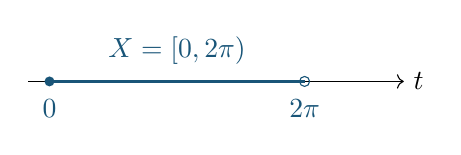
\begin{tikzpicture}[scale=0.9]
    \draw[->] (-0.3,0) -- (5,0) node[right]{$t$};
    \draw[very thick, defcolor] (0,0) -- (3.6,0);
    \fill[defcolor] (0,0) circle (2pt) node[below=3pt]{$0$};
    \draw[defcolor] (3.6,0) circle (2pt) node[below=3pt]{$2\pi$};
    \node[defcolor, above] at (1.8,0.1) {$X=[0,2\pi)$};
  \end{tikzpicture}
  \end{center}
  \column{0.46\textwidth}
  \begin{center}
  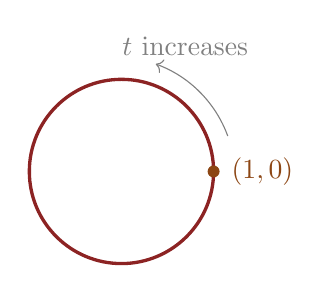
\begin{tikzpicture}[scale=0.9]
    \draw[very thick, thmcolor] (0,0) circle (1.3);
    \fill[mAccent] (1.3,0) circle (2.4pt);
    \node[mAccent, right=3pt] at (1.3,0) {$(1,0)$};
    \draw[->, gray] (1.5,0.5) arc (20:70:1.7);
    \node[gray, above] at (0.9,1.5) {$t$ increases};
  \end{tikzpicture}
  \end{center}
  \end{columns}
  \vspace{1.0em}
  \begin{center}
  \begin{hlbox}
  Points just \emph{below} $2\pi$ map near $(1,0)$, but their
  preimages are far from $0$ --- the inverse \alert{tears} the circle.
  \end{hlbox}
  \end{center}
  \note{
    On the left is the domain, the half open interval from zero to two pi,
    with a solid dot at zero included and an open dot at two pi excluded. On
    the right is the unit circle, the image. As "t" increases from zero, the
    point travels counterclockwise around the circle and returns toward the
    starting point one comma zero, marked in orange. Here is the trouble.
    Inputs just below two pi land very close to one comma zero on the
    circle, and so does the input zero itself. So nearby outputs on the
    circle can come from inputs near two pi and from inputs near zero, which
    are far apart in the domain. The inverse must therefore tear the circle
    open at the seam, and that tearing is exactly a discontinuity. Note the
    circle "Y" is compact, yet the inverse still fails, because it is the
    domain that must be compact.
  }
\end{frame}

% =============================================================================
}

{
\usebackgroundtemplate{%
  
\includegraphics[width=\paperwidth,height=\paperheight,keepaspectratio=false]{chapter_04_bg_08.png}%
}
\section{Summary}
% =============================================================================

% --- Build 1/4 ---
\begin{frame}{Summary}
  \begin{hlbox}
  \textbf{Key takeaways:}
  \begin{itemize}
    \item \alert{Theorem 4.14:} continuity preserves compactness ---
      $f(X)$ is compact.
  \end{itemize}
  \end{hlbox}
  \note{
    Let us gather everything together. The cornerstone of the section is
    Theorem 4.14: a continuous function maps compact sets to compact sets.
    Continuity preserves compactness. Every other result we proved flows
    from this single fact. Let's recall those consequences.
  }
\end{frame}

% --- Build 2/4 ---
\begin{frame}{Summary}
  \begin{hlbox}
  \textbf{Key takeaways:}
  \begin{itemize}
    \item \alert{Theorem 4.14:} continuity preserves compactness ---
      $f(X)$ is compact.
    \item \alert{Theorem 4.16:} a continuous real function on a compact set
      \emph{attains} its max and min.
  \end{itemize}
  \end{hlbox}
  \note{
    From the cornerstone we obtained the extreme value theorem, Theorem
    4.16. A continuous real valued function on a compact domain does not
    merely stay bounded; it actually achieves a largest value and a smallest
    value at genuine points of the domain. This is one of the most used
    theorems in analysis and optimization. Next, the inverse and uniform
    continuity results.
  }
\end{frame}

% --- Build 3/4 ---
\begin{frame}{Summary}
  \begin{hlbox}
  \textbf{Key takeaways:}
  \begin{itemize}
    \item \alert{Theorem 4.14:} continuity preserves compactness ---
      $f(X)$ is compact.
    \item \alert{Theorem 4.16:} a continuous real function on a compact set
      \emph{attains} its max and min.
    \item \alert{Theorems 4.17 \& 4.19:} continuous bijections invert
      continuously; continuity becomes \emph{uniform}.
  \end{itemize}
  \end{hlbox}
  \note{
    Two more corollaries. Theorem 4.17 says a continuous one to one map from
    a compact space onto another space has a continuous inverse, so it is a
    homeomorphism. And Theorem 4.19 says continuity on a compact domain is
    automatically uniform continuity, with the finiteness of a subcover
    being the decisive ingredient. Finally, a word on why compactness was
    indispensable.
  }
\end{frame}

% --- Build 4/4 ---
\begin{frame}{Summary}
  \begin{hlbox}
  \textbf{Key takeaways:}
  \begin{itemize}
    \item \alert{Theorem 4.14:} continuity preserves compactness ---
      $f(X)$ is compact.
    \item \alert{Theorem 4.16:} a continuous real function on a compact set
      \emph{attains} its max and min.
    \item \alert{Theorems 4.17 \& 4.19:} continuous bijections invert
      continuously; continuity becomes \emph{uniform}.
    \item \alert{Theorems 4.20--4.21:} drop compactness and every result
      can fail.
  \end{itemize}

  \vspace{0.4em}
  \textbf{Coming up next:} \emph{Continuity and Connectedness}.
  \end{hlbox}
  \note{
    And the counterexamples of Theorem 4.20 and Example 4.21 show the
    hypotheses cannot be weakened. On a noncompact set we can find
    continuous functions that are unbounded, that have no maximum, or that
    are not uniformly continuous, and a continuous bijection whose inverse
    is discontinuous. Compactness is genuinely doing the work. In the next
    section we pair continuity with the other great topological property,
    connectedness, and we will recover the intermediate value theorem.
    Thanks for watching, and see you there.
  }
\end{frame}
}

\end{document}
